\section{Spectrecoin Basic Properties}
The Spectrecoin software is encompassing and integrating the following:

\begin{itemize}
	\item Bitcoin Core (core technology of the Spectrecoin block-chain)
	\item Proof-of-Stake.v3 (PoSv3) (secure ‘open’ consensus mechanism for XSPEC public coins)
	\item Proof-of-Anonymous-Stake (PoAS) (secure private consensus mechanism for SPECTRE private coins)
	\item Private transactions (using dual-key stealth technology and ring signatures for SPECTRE)
	\item TOR to hide your real IP address (all Spectrecoin nodes run as hidden services)
	\item OBFS4 to hide the fact that you are using TOR to avoid censorship
\end{itemize}



\subsection{Core Specification}

\begin{tabulary}{\textwidth}{L|J}
	\hline
	Genesis block 				& Block \#1 mined on 20/11/2016 (later transition to PoS only)\\
	\hline
	Distribution  				& ICO that raised 16 BTC w/ subsequent distribution in early 2017\\
	\hline
	Ticker 						& XSPEC\\
	\hline
	Initial supply 				& 20,000,000 XSPEC\\
	\hline
	Network outputs (public) 	& XSPEC – public coins\\
	\hline
	Network outputs (private)	& SPECTRE – private coins\\
	\hline
	Consensus (XSPEC) 			& Proof-of-Stake v.3 (PoSv3)\\
	\hline
	Consensus (SPECTRE) 		& Proof-of-Anonymous-Stake (PoAS)\\
	\hline
	Difficulty retarget 		& Every block\\
	\hline
	Target block time 			& 96 seconds\\
	\hline
	Block reward (PoSv3) 		& 2 XSPEC\\
	\hline
	Block reward (PoAS) 		& 3 SPECTRE\\
	\hline
	Coin maturity (confirmations) 	& 450 for stake reward / 10 for SPECTRE / 6 for XSPEC\\
	\hline
	Max supply 					& No max supply (see illustrations on page 8)\\
	\hline
	Inflation 					& Decreasing over time tending to zero\\
	\hline
	Code repository 			& https://github.com/spectrecoin/spectre\\
	\hline
	Supported platforms / OS 	& MS Windows, OSX, Linux, Raspberry Pi\\
	\hline
	Website 					& https://spectreproject.io/\\
	\hline
	Block explorer 				& https://chainz.cryptoid.info/xspec/\\
	\hline
\end{tabulary}

\pagebreak[4]

It is important to understand that the total ‘outstanding’ amount is the sum
of XSPEC + SPECTRE. On the next page we have projected both a minimum and a
maximum inflation rate and total ‘outstanding’ amount of XSPEC + SPECTRE over
20 years. The real value of the total ‘outstanding’ amount will depend on the
ratio of XSPEC / SPECTRE created by the two different consensus mechanisms
over time. The minimum values represent a scenario where 100\% of the blocks
are created by PoSv3 and the maximum values represent a scenario where 100\%
of the blocks are created by PoAS.

\begin{figure}
	\centering
	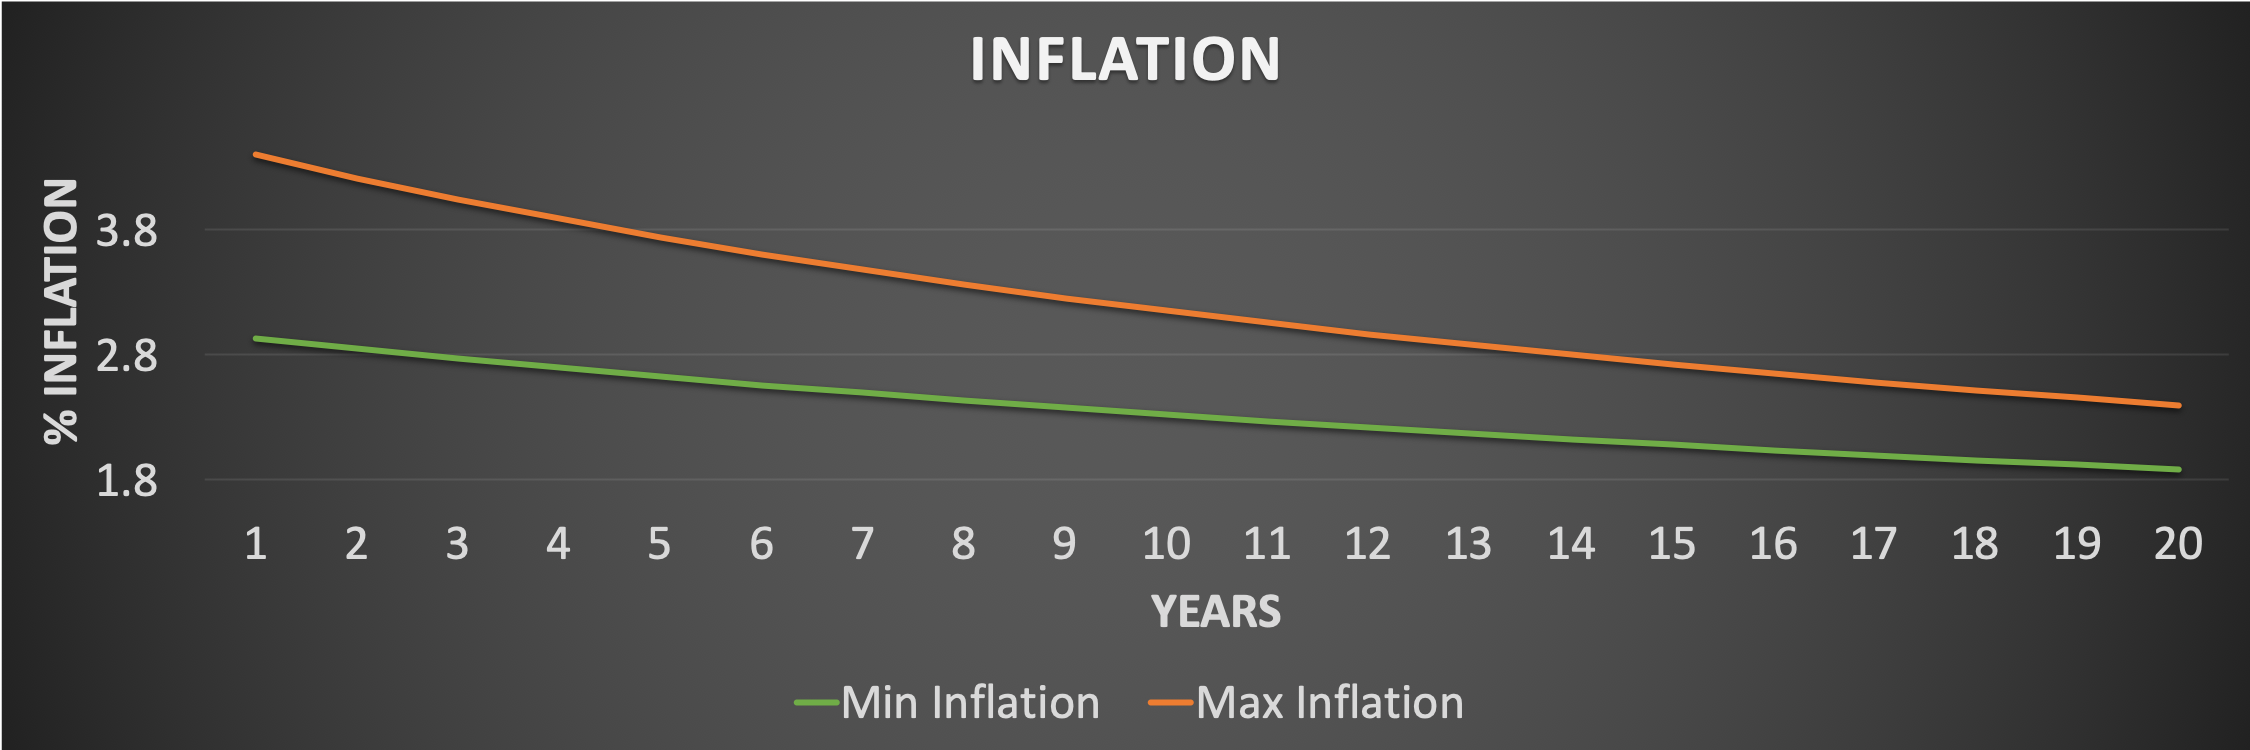
\includegraphics[width=\textwidth]{inflation.png}
	\caption{Min inflation rate after 20 years = 1.88 - Max inflation rate after 20 years = 2.40 }
	\centering
	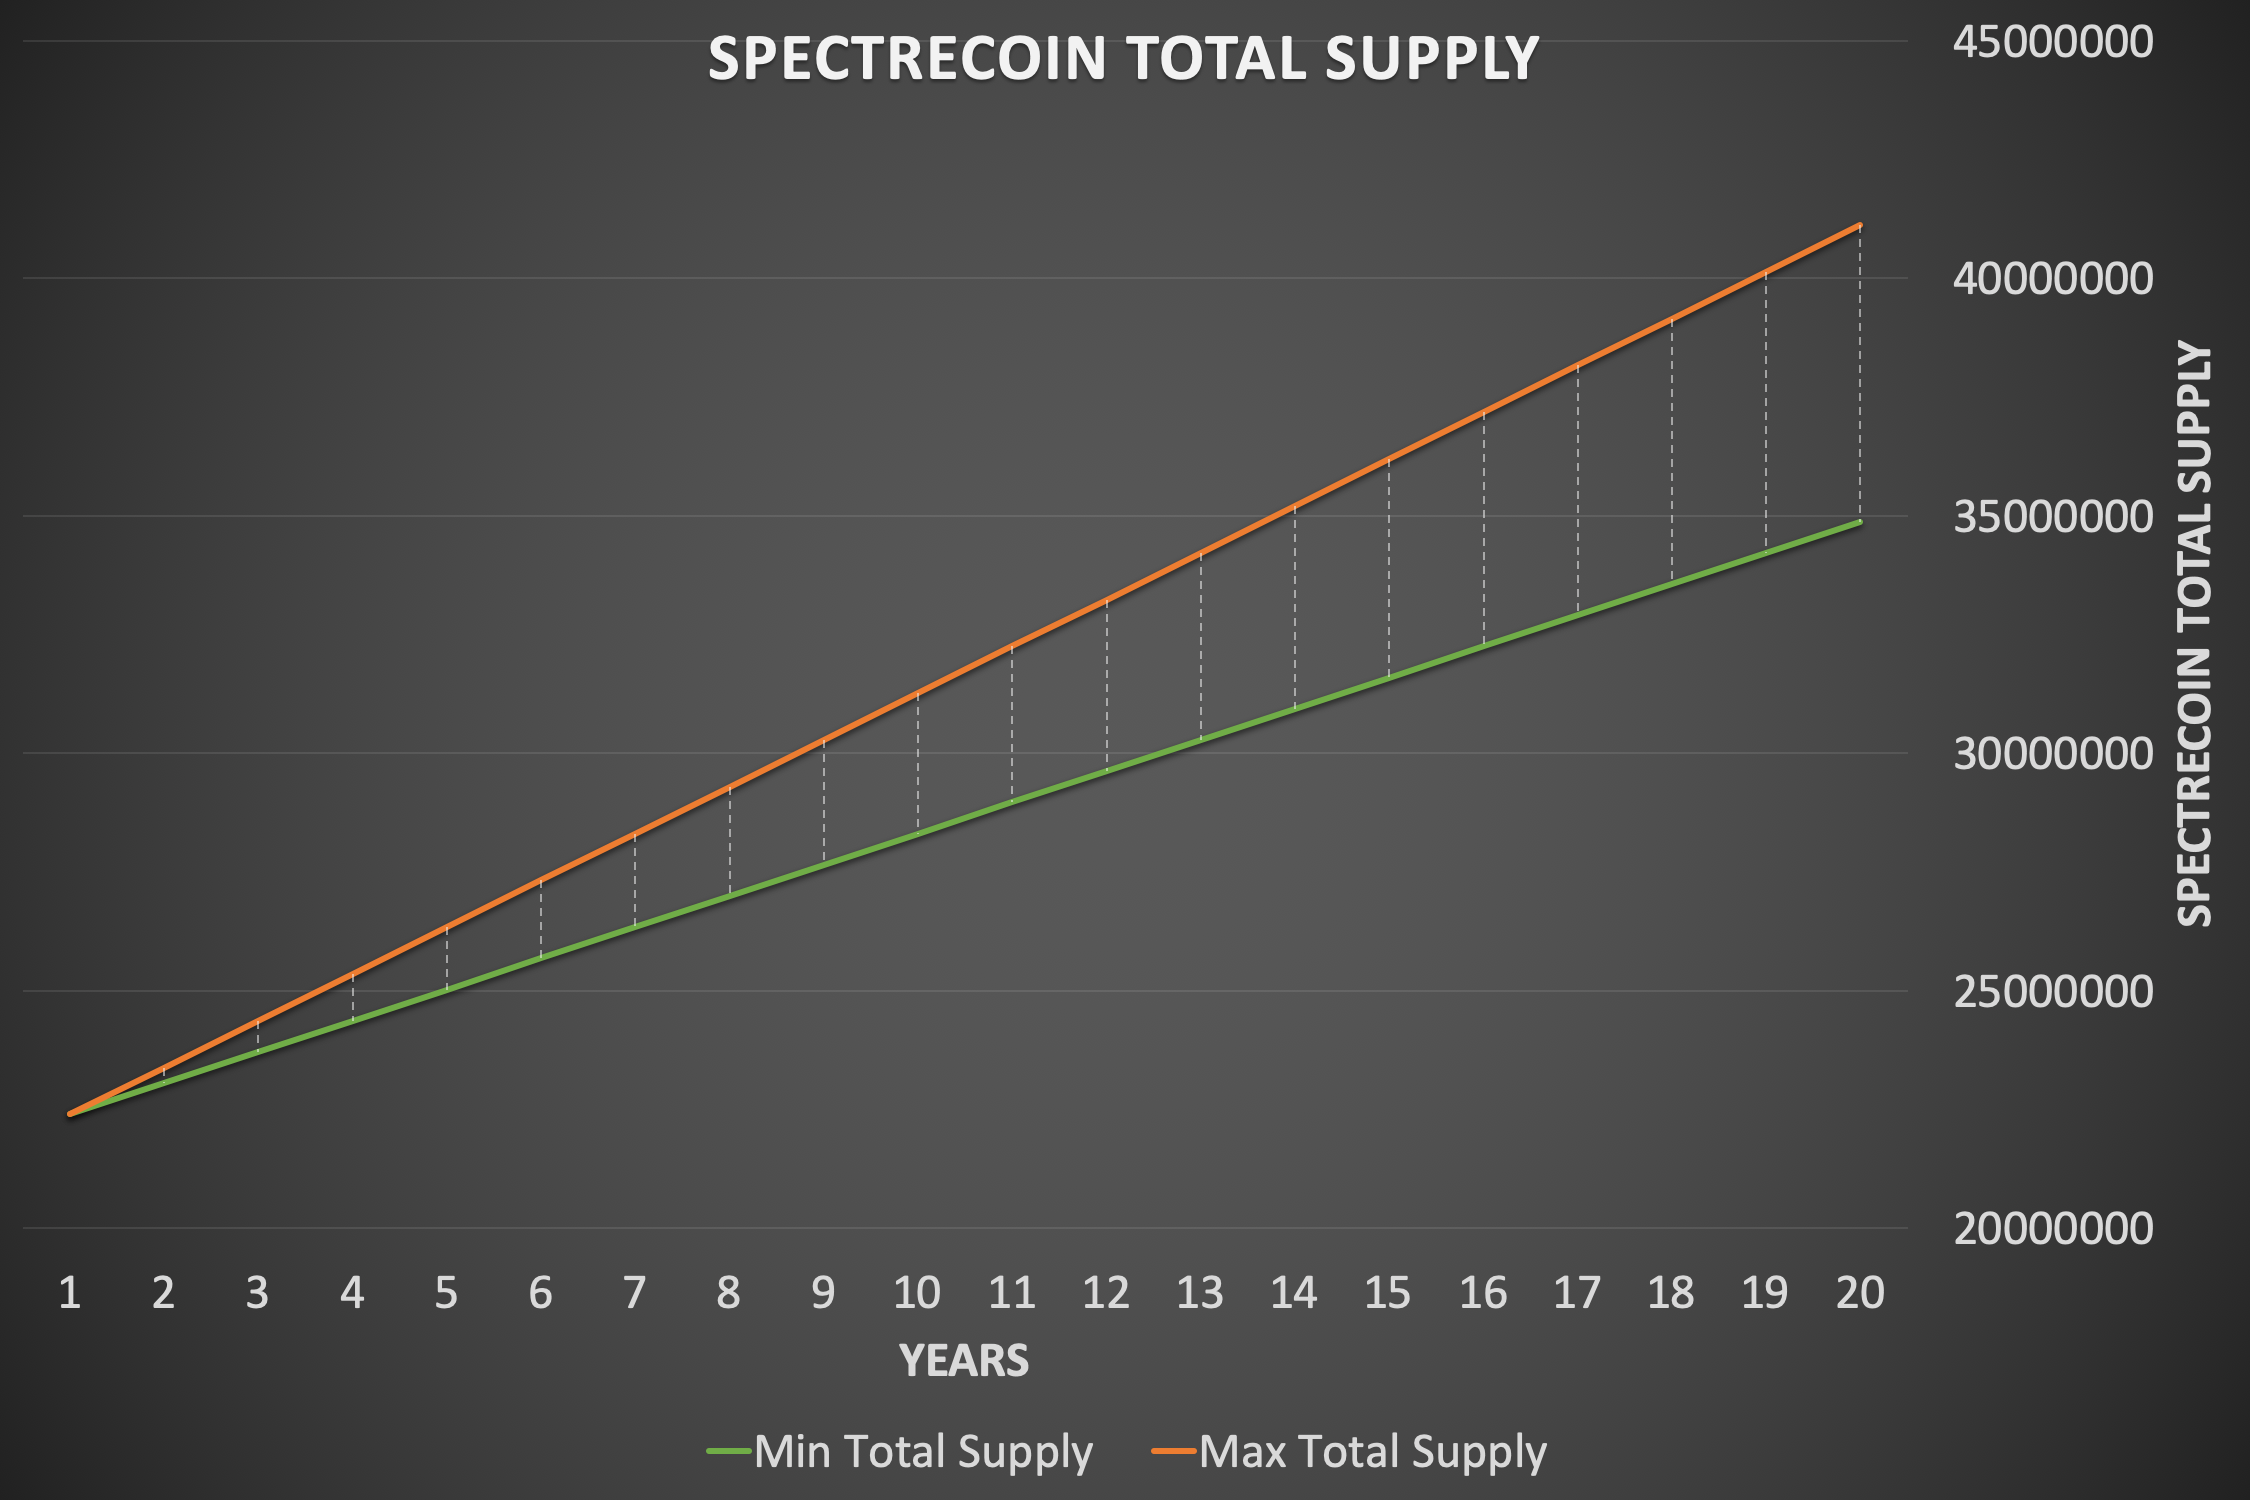
\includegraphics[width=\textwidth]{supply.png}
	\caption{}
\end{figure}



\subsection{Maturity}
The maturity calculations have changed such that the minimum maturity for
staking and for spending stakes has been increased from 288 to 450 blocks.
This is approximately 96 seconds * 450 = 12 hours and hence the 8-hour
maturity rule for staking has been removed. Also, note that the updated
maturity rule is also considered for all ATXOs used in the ring signature
of the staked VIN.



\subsection{Reward and Fee Handling}
The stake reward for a PoAS block is 3 SPECTRE and 2 XSPEC for a PoSv3 block.
The fees are the same for both XSPEC and SPECTRE transactions.



\subsection{Proof-of-Stake vs. Proof-of-Work}
Spectrecoin uses both PoSv3 and PoAS algorithms to keep the network consensus
and to secure and confirm transactions. Both PoSv3 and PoAS appear to be more
resilient against various attacks that could be instigated against a
Proof-of-Work (PoW) system like Bitcoin, Litecoin and DASH for example.
It is also known that PoW systems are susceptible to so called 51\% attacks
where a sufficiently funded and motivated attacker can “take control” over
the network and generate double spend transactions12. It is more difficult
to attack a PoS system in this way as it would be infeasible to acquire the
majority of Spectrecoin in circulation and doing so would undermine the value
and remove the incentive for the attack in the first place. There are obviously
other attack vectors, such as the recently discovered so called “Fake Stake”
attack against PoSv313. This has since been fixed by the Spectrecoin developers
and Spectrecoin is no longer susceptible to such an attack.



It is also well known that large PoW driven networks expend huge amounts of
energy and appears to lead to some level of centralisation of mining power
due to the huge expense involved in mining new blocks. In a recent research
paper entitled “The Bitcoin Mining Network - Trends, Composition, Average
Creation Cost, Electricity Consumption \& Sources” by Christopher Bendiksen
\& Samuel Gibbons of CoinShares Research14, it was found that the Bitcoin
network expends more energy than the whole country of New Zealand.



The report calculated that the global Bitcoin mining industry draws 4.7GW of
power every second. Hashing computations for the Proof-of-Work algorithm
consumed 4.3GW, up 0.4GW from the last CoinShares report in November 2018.
Based on these figures, researchers calculated an annual consumption of
41TWh of electricity. That’s roughly 2.2TWh more than New Zealand – a country
of 4.7M people – consumed in 2017, according to the country’s Electricity
Authority15.



In comparison, Spectrecoin will run on a standard Raspberry Pi and in addition
to all the privacy features, Spectrecoin is also truly eco-friendly, sustainable
and ‘green technology’. The estimated loose upper bound, annual consumption for
a Raspberry Pi running Spectrecoin is 16.6kWh.

\vspace{5mm} %5mm vertical space

Bitcoin network:\\
$41 TWh = 41*1012 Wh = 41,000,000,000,000 Wh$

\vspace{5mm} %5mm vertical space

Spectrecoin node:\\
$16.6 KWh = 16.6 * 103 Wh = 16,600 Wh * 1000 (nodes) = 16,600,000 Wh$

\vspace{5mm} %5mm vertical space

That means that the whole Bitcoin network consumes almost 2.5 million times
more energy than what an imaginary Spectrecoin network would consume, assuming
1000 Spectrecoin Raspberry Pi nodes.




In summary, the PoSv3 / PoAS protocols are both potentially more secure,
immensely more energy efficient and provides for better decentralisation.
It is beyond the scope of this paper to discuss this further and there are
various discussions around the internet if you are interested in the PoW vs.
PoS debate.



In the next sections we will explore the different aspects of Spectrecoin in
more detail. We start on the next page with a detailed introduction to the
Spectrecoin privacy features before we go on to discuss Proof-of-Stake v3
(PoSv3) in detail. We move on to explain the privacy features and the new
Proof-of-Anonymous-Stake (PoAS) protocol.